\documentclass[english,11pt,a4paper]{article}
\usepackage{preamble}

%-------------------------------------------------------------------------%
% MASTERARBEIT (╯°□°)╯︵ ┻━┻       ┬─┬ノ( º _ ºノ)      (ノಠ益ಠ)ノ彡┻━┻   %
%
%                (ノ`Д´)ノ彡┻━┻                  ┬─┬ノ( º _ ºノ)
%-------------------------------------------------------------------------%

\begin{document} %------------   \(◕ ◡ ◕\)   -----------------------------%
% (/◔ ◡ ◔)/   ◕‿◕



\newpage

Version 6 \scriptsize \hfill Juri; Hyperelliptic Curves --- Draft --- \today
\normalsize

\section{Addition Law}\label{ch1}

\subsection{Definitions and Notation}

\begin{defin}
  Let $K$ be a field with char$(K) \neq 2, 3$ and $\bar K$ its algebraic closure. Define the hyperelliptic curve of genus two $\enk$ as the set of solutions in $K^2$ to the equation $y^2=C(x)$ where
  \begin{align*}
    C(x)=x^5+ax^4+bx^3+cx^2+dx+e
  \end{align*}
  is a polynomial over $K$. Similarly, the set of solutions in the closure would be denoted $\enkb$.  Define $\ek$ as $\enk \cup \{ \infty \}$.

  \textbf{Note} that we could obtain a more reduced form of $C(x)$, eliminating $a$ by shifting $x$ to $x-a/5$. However, since this would rob us of the possibility of char$(K) = 5$ without simplifying our coming calculations in any significant manner, we shall be reluctant towards using this trick.

  For the purpose of clarity, let points on the hyperelliptic curve --- in the sense of solutions to $y^2=C(x)$ --- be designated by the calligraphic letter $\q=(x,y) \in \enkb$. The point opposite to $\q$ will be written $\bar \q = (x,-y)$ and by symmetry of the curve in $y$ also belongs to $\enkb$. In the case where $\q = \infty$, define $\bar \q = \infty$.

  We then want to consider the set of all pairs $(\q_1,\q_2)$ and tame it with an equivalence relation with the goal of obtaining an additive group:
\end{defin}
% \vspace{2mm}
\begin{defin}\label{defj}
  Define $\J$ to be the set\scalebox{1.3}{ $\nicefrac{ \j }{\sim }$ }where $\j = \ekb \times \ekb$. It is called the ``Jacobian'' and the equivalence relation is defined by
  \begin{align*}
    (\q_1,\q_2) &\sim (\q_2,\q_1) \\
    \text{and\hspace{5mm}} (\q,\bar \q) & \sim ( \infty , \infty ). 
  \end{align*}
  Write $\{ \q_1,\q_2 \}$ from now on and let bold letters denote points on the curve in the sense of classes of unordered pairs $\P =\{ \q_1, \q_2 \} \in \J$. The point $\{ \bar \q_1, \bar \q_2 \}$ will be called $\bar \P$ for now but can already tentatively be thought of as $-\P$. Call $\{ \infty, \infty \}$ the zero of our set. Call $\q_i$ a point-component.

  A point $\q = (x_0,y_0)$ is called singular if it fulfills both $y_0=0$ and $C'(x_0) = 0$. A curve is called singular if and only if it has a singular point. We consider only non-singular hyperelliptics from here on; this amounts to $C(x)$ having no repeated factors over $\bar K$ (``squarefree'').
\end{defin}

\subsection{The General Case}

Let's start with $\P_1 = \{\q_1,\q_2\}$, $\P_2 = \{\q_3,\q_4\}$ with $\q_i = (x_i,y_i) \in \enk$ or $\q_i = \infty$. To define $\P_3 = \P_1 + \P_2$ we distinguish between one general case and a number of special cases and first derive the results of the former before enumerating the latter ones.

\begin{case} {\scshape Four Distinct Point-Components:}
  Let $\q_i \in \enk$ and $\P_i$ be defined as above with $x_i \neq x_j$ whenever $i \neq j$.

  The overarching idea is to obtain a fifth and sixth $x$-coordinate and the corresponding $y$-coordinates by passing a polynomial of degree three through the four points $\q_i$. Ideally this should give us two additional intersections with the curve which we then use as the components of our point $\P_1 + \P_2$.

  {\scshape Step 1:} It is known that the Vandermonde matrix
  \begin{align*}V=
    \begin{pmatrix}
      1 & x_1 & x_1^2 & x_1^3\\
      1 & x_2 & x_2^2 & x_2^3\\
      1 & x_3 & x_3^2 & x_3^3\\
      1 & x_4 & x_4^2 & x_4^3\\
    \end{pmatrix}
  \end{align*}
  has determinant $\prod_{i < j} (x_i-x_j)$ which is conveniently non-zero if and only if the $x_i$ are pairwise distinct. Let $P(x) = p_3 x^3 + p_2 x^2 + p_1 x + p_0 \in \bar K[x]$ be the polynomial in unknown coefficients that we are looking for. With $\textbf{y} = (y_1 \ y_2 \ y_3 \ y_4)^t$ and $\textbf{p} = (p_0 \ p_1 \ p_2 \ p_3)^t$, the problem of determining $P(x)$ can be rewritten as
  \begin{align*}
    V \cdot \mathbf{p} = \mathbf{y}
  \end{align*}
  which by invertibility of $V$ has a unique solution for $\mathbf{p}$ with $p_i\in K$.

  \textbf{Note} that the leading coefficient of $P(x)$ is
  \begin{align*}
    p_3 = \frac{1}{\det (V)}
    \begin{vmatrix}
      1 & x_1 & x_1^2 & y_1\\
      1 & x_2 & x_2^2 & y_2\\
      1 & x_3 & x_3^2 & y_3\\
      1 & x_4 & x_4^2 & y_4\\   
    \end{vmatrix}
  \end{align*}
  and the next step will depend on whether $P(x)$ is truly of degree 3 or not.\vspace{-1mm}
\fline
\vspace{-2.5mm}
  \begin{align*}\tag{$\ast$} \label{sex}
    \rlap{\hspace{-44.5mm} Define}
    D(x) = C(x)-\left ( P(x) \right )^2.
  \end{align*}\vspace{-5mm}
  \hrule

  {\scshape Step 2a:} Knowing the coefficients $p_i$ we first assume $p_3 \neq 0$ so we can proceed to look for the additional solutions of the sextic equation $D(x) = 0$.
  Observe that this vanishes at $x_1, x_2, x_3$ and $x_4$, so write the lefthand side as
  \begin{align}\tag{$*_1$}
    D(x) = -p_3^2(x-x_1)(x-x_2)(x-x_3)(x-x_4)(x-x_5)(x-x_6)
  \end{align}
   for $x_5$ and $x_6$ unknowns in $\bar K$. Comparing the coefficients at $x^4$ and $x^5$ yields
  \begin{align*}
    \sum_{\substack{i,j=1\\i<j}}^6 x_i x_j &= T_4\\
    \rlap{\hspace{-56mm}and} \sum_{i=1}^6 x_i &= T_5
  \end{align*}
  where $T_4 = \frac{p_2^2+2 p_1 p_3-a}{p_3^2}$ and $T_5 = \frac{1-2 p_2 p_3}{p_3^2}$.
  The first expression gives
  \begin{align*}
    x_6 \sum_{i=1}^5 x_i + \sum_{\substack{i,j=1\\i<j}}^5 x_i x_j = T_4.
  \end{align*}
  Replacing $x_6$ by $T_4 - \sum_{\substack{i,j=1\\i<j}}^5 x_i x_j$ gives the tidy quadratic equation

  \vspace{-2mm}
  \fline
  \begin{align*}
    \tag{$\dag$} \label{dagger} x^2 - \left(T_5 - \sumfo \right) \cdot x+ \left(T_4 - T_5 \sumfo + \sum_{\substack{i,j=1\\i\leq j}}^4 x_i x_j \right) = 0
  \end{align*}
  \fline

  of which $x_5$ is one solution and --- by symmetry of the above steps --- $x_6$ the other one. Compute $y_i=P(x_i)$ for $i=5,6$ to obtain $\q_5 = \{ x_5, y_5 \}$ and $\q_6 = \{ x_6, y_6 \}$, at which point it becomes clear that the worst-case scenario for our field extension to accommodate the new coordinates is to be quadratic. Finally we define $\P_1 + \P_2$ to be equal to $\P_3 = \{ \bar \q_5, \bar \q_6 \}$.

  {\scshape Step 2b:} If $p_3$ were zero, the equation \eqref{sex} would be quintic instead. We may therefore write the lefthand side factorized, so we get a different $D(x)$,
  \begin{align}\tag{$*_1$}
  D(x) = (x-x_1)(x-x_2)(x-x_3)(x-x_4)(x-x_5),
  \end{align}
  again for $x_5$ somewhere in $\bar K$. We used the tag ($*_1$) twice to refer to  both equations. Defining $T_{4\infty}=p_2^2 - a$ and comparing the coefficients at $x^4$ gives

  \vspace{-3mm}
  \fline
  \begin{align*}
    \tag{$\ddag$} \label{dagger2} x_5 = T_{4\infty} - \sum_{i=1}^4 x_i
  \end{align*}
  \fline

  and we may rejoice in the implication of $x_5$ staying in $K$.

  Compute $y_5 \hspace{-0.8mm} = \hspace{-0.8mm} P(x_5)$ and define $\P_1 + \P_2$ to be the point $\P_3 = \{ (x_5, -y_5), \infty \}$.

  {\scshape Step $1'$:} To extend our construction from $\enk$ to $\ek$ we now consider $\q_4 = \infty$ with the other $\q_i = (x_i,y_i)$ as before. This can be seen as the $x_i$ still being pairwise distinct, only that one of them is allowed to be $\infty$ here.

  There is no coordinate $x_4$ this time, so we pass a quadratic polynomial $P(x)$ through the remaining three points $(x_i,y_i)$. This means that we solve the linear system $\tilde V \cdot \mathbf{p} = \tilde \mathbf{y}$ where $\tilde V$ is the Vandermonde matrix for $x_i$, $i=1,..,3$,
  \begin{align*}\tilde V=
    \begin{pmatrix}
      1 & x_1 & x_1^2\\
      1 & x_2 & x_2^2\\
      1 & x_3 & x_3^2\\
    \end{pmatrix}
  \end{align*}
  As before, the leading coefficient of $P(x)$ might or might not be zero, 
  %but this time, dear reader, let us not give a toss
  but \eqref{sex} will be quintic in either case, so we only have to worry about one step 2.

  {\scshape Step $2'$:} Doing a coefficient comparison at $x^3$ and at $x^4$ in \eqref{sex} through
  \begin{align*}\tag{$*_1'$}
    D(x) = (x-x_1)(x-x_2)(x-x_3)(x-x_5)(x-x_6),
  \end{align*}\vspace{-8mm}
  \begin{align*}
    \rlap{\hspace{-21mm} gives}
    \sum_{\substack{i,j=1\\i<j}}^3 x_i x_j + x_5\sum_{i=1}^3 x_i + x_6\sum_{i=1}^3 x_i + x_5 x_6 &= b-2p_1 p_2\\
    \rlap{\hspace{-59mm} and}
    \sum_{i=1}^3 x_i + x_5 + x_6 &= p_2^2-a.
  \end{align*}
  Call the righthand terms $T_{3\infty}$ and $T_{4\infty}$, combine both equations and obtain

  \vspace{-2mm}
  \fline
  \begin{align*}
    \label{daggerp} \tag{$\dagger '$} x^2 - \left( T_{4\infty} - \sumthr \right) \cdot x + \left(T_{3\infty} - T_{4\infty} \sumthr + \sum_{\substack{i,j=1\\i\leq j}}^3 x_i x_j \right)
  \end{align*}
  \fline

  Solve, call the two solutions $x_5$ and $x_6$, compute $y_5$ and $y_6$ through $P(x_5)$ and $P(x_6)$ and define $\P_1+\P_2$ to be $\P_3=\{ (x_5,-y_5) , (x_6,-y_6) \}=\{ \bar \q_5, \bar \q_6 \}$.
\end{case}


\begin{figure}[ht!]
  \fline
  \begin{center}
    \vspace{1mm}
    % \framebox{The eight cases illustrated}
    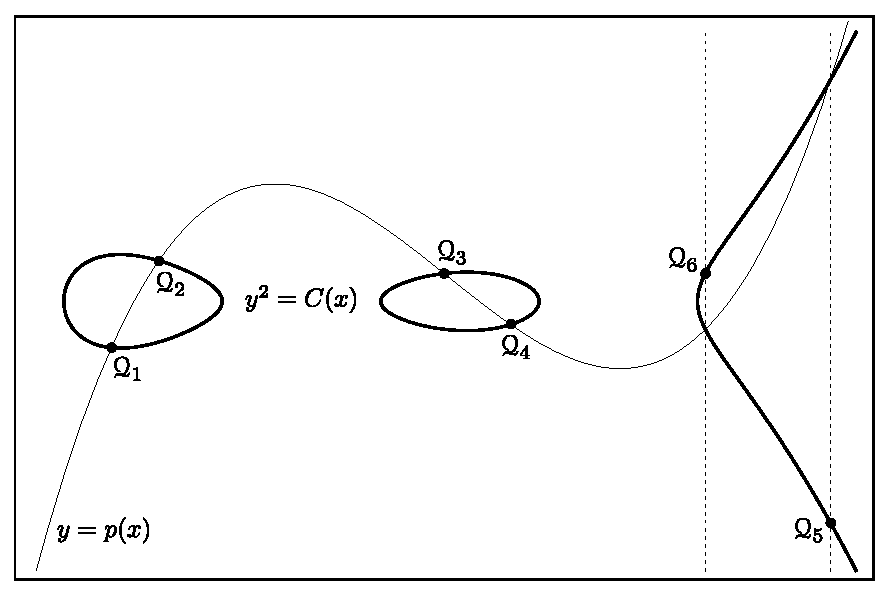
\includegraphics[width=0.9\textwidth]{addition_general.pdf}

    {\scshape Figure 1a}: The general case for the addition law in $\mathds{R}^2$ where $p_3 \neq 0$.

    \vspace{1mm}

    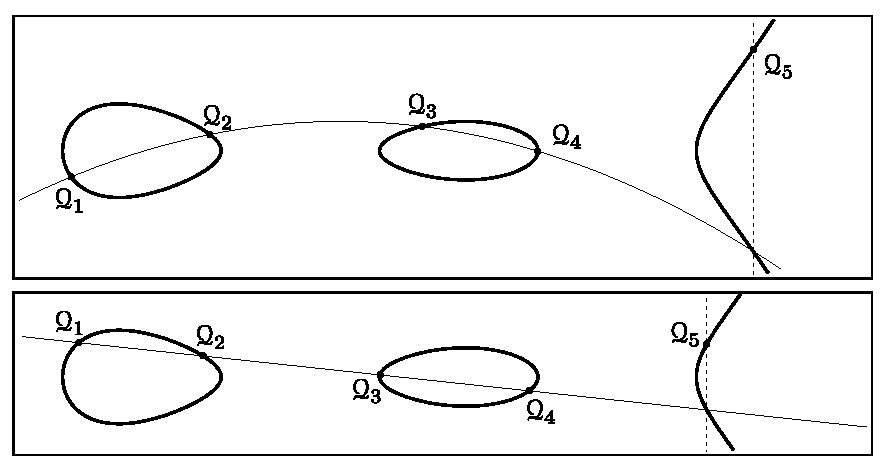
\includegraphics[width=0.9\textwidth]{addition_quadr_and_lin.pdf}

    {\scshape Figures 1b} and {\scshape 1c}: If $p_3 = 0$ we have exactly five finite intersections.
  \end{center}
  \vspace{-1.5mm}
  \fline
\end{figure}


\begin{remark}
  Up to this point, we have given the general-case rule only for elements in $\ek \times \ek$. Extending to $\j = \ekb \times \ekb$ is trivial as we can simply choose $\bar K$ as the new $K$. The final step is to note that everything until now is well-defined on $\J$. The equivalence relation from Definition \ref{defj} corresponds to interchanging $\q_1$ and $\q_2$ or $\q_3$ and $\q_4$ or both.
  To this end we can check that interchanging $(x_i,y_i)$ and $(x_j,y_j)$ does nothing to the resulting $\q_5$ and $\q_6$. This is the case because $P(x)$ depends only on the solution of the linear system $V \cdot \mathbf{p} = \mathbf{y}$ on which the aforementioned permutation has no effect. With $p$ invariant, the subsequent steps remain unchanged as well.

  Finally, the restriction to $K$ instead of $\bar K$ was to showcase the degree of the required field extension, a feat we will now leave aside by always using $\bar K$.
\end{remark}


%\textbf{Note} also that solving either of the dagger equations does not guarantee that the resulting $x_5$ or $x_6$ differ from the other $x_i$ or even from each other. In fact the situation may very well arise where for instance $x_6 = x_1$ because $P(x)$ happens to be tangential to the curve at $x_1$. The equation \eqref{sex} would then factor as $-p_3^2(x-x_1)^2\prod_{i=1}^5 (x-x_i)$.

% \newpage
Before we begin listing the special cases, we impose the following property: The sum of any $\P_1 = \{\q_1,\q_2\}$ and $\P_2 = \{\q_3,\q_4\}$ in $\J$ fulfills the equality
\begin{align*}
  \tag{$\diamondsuit$} \label{switch} \P_1 + \P_2 &= \{\q_3,\q_2\} + \{\q_1,\q_4\}.
\end{align*}
Note that the general-case addition we just defined already fulfills this, as we noted before that interchanging any of the $(x_i, y_i)$ does not impact the solution $\mathbf{p}$ of the linear system nor any of the dagger equations.

\begin{remark}\label{permut}
  The property \eqref{switch} corresponds to the permutation $(1 \, 3)$ on the point-components $\q_i$. With Definition \ref{defj} allowing the permutations $(1 \, 2)$ and $(3 \, 4)$ this naturally leads to the observation that in fact all permutations of point-components must now leave the sum unchanged. In fact it is easy to check that the three transpositions generate all of $S_4$ and the remark above already provides compatibility with the construction of the general case.

  A substantial bonus of this is the fact that commutativity corresponds to the permutation $(1 \, 3)(2 \, 4)$ which by the above we now obtained for free.
\end{remark}

% \newpage

\subsection{Complete List of Cases}

We may now impose conditions on the relations between the $\q_i$ without mentioning whether they belong to $\P_1$ or $\P_2$. As a result, the list of special cases can be written in a significantly more concise manner.

As we strive to define $\{ \q_1 , \q_2 \} + \{ \q_3 , \q_4 \}$, for any $\q_i = (x_i,y_i) \in \enkb$ or $\q_i = \infty \in \ekb$ we observe that the following simplification takes place:

Let $\{ i,j,k,l \}=\{ 1,2,3,4 \}$. Whenever $\q_i = \bar \q_j$ for $i \neq j$ we have
\begin{flalign*}
  && \{ \q_1 , \q_2 \} + \{ \q_3 , \q_4 \}
            &= \{ \q_i , \q_j \} + \{ \q_k , \q_l \} &\\
  &&        &= \{ \q_k , \q_l \} + \{ \q_j , \bar \q_j \} &\\
  \label{zero}\tag{0}
  &&        &= \{ \q_k , \q_l \} + \{ \infty, \infty \} = \{ \q_k , \q_l \}
\end{flalign*}
The justification for this follows directly from Remark \ref{permut} and Definition \ref{defj}. It is easily checked that this sum remains well defined if the choice of $i$ and $j$ is not unique. This allows us to treat the above as a separate case in order to characterize the other cases solely through the $x$-coordinates of the $\q_i$, so we may assume
\begin{align*}
  x_i = x_j \iff \q_i = \q_j
\end{align*}
for any $\q_i, \q_j \in \ekb$, provided we assign $\q_i = \infty$ the $x$-coordinate $x_i = \infty$. 
There is a possibility for ambiguity of ``$\infty$'' here, which we will however avoid later on by making it obvious which infinity we are working with.

We may now write the distinction between the remaining cases as follows:

\begin{enumerate}
  \parskip 1mm
  \item The general case where $x_1,x_2,x_3,x_4$ are pairwise distinct.
  \item The case where exactly two of $x_1,x_2,x_3,x_4$ are equal.
  \item The case where $x_1,x_2,x_3,x_4$ are equal in pairs.
  \item The case where exactly three of $x_1,x_2,x_3,x_4$ are equal.
  \item The case where where all of $x_1,x_2,x_3,x_4$ are equal.
\end{enumerate}
\parskip 3mm


\newpage

Since we are allowed to permute point-components anyway, we may fix which of the $\q_i$ are equal and write everything out for the complete and final list.

\begin{center}
  Given the addition $\{ \q_1 , \q_2 \} + \{ \q_3 , \q_4 \}$, distinguish between the following:
\end{center}

\vspace{-3mm}
\fline
\begin{enumerate}\setcounter{enumi}{-1}
  \parskip 1mm
  \item The addition with zero, i.e. $\q_1 = \bar \q_2$ with $\q_i \in \ekb$ for $i = 1,..,4$.
  \item The general case where $\q_i \neq \q_j$ and $\q_i \neq \bar \q_j$ for $i \neq j$.
  \item The single tangential case where all $\q_i$ as in case 1 with the exception of $\q_1 = \q_2 \in \enkb$ with $y_1 \neq 0$.
  \item The double tangential case where all $\q_i$ as in case 1 with the exception of $\q_1 = \q_2 \in \enkb$ with $y_1 \neq 0$ and $\q_3 = \q_4 \in \enkb$ with $y_3 \neq 0$.
  \item The triple point case wherein $\q_1=\q_2=\q_3 \in \enkb$ with $y_1 \neq 0$ and $\q_4 \in \ekb$ differs from both $\q_1$ and $\bar \q_1$.
  \item The quadruple point case where all $\q_i \in \enkb$ are equal with $y_1\neq 0$.
\end{enumerate}
\vspace{-2mm}
\fline
\parskip 3mm

\begin{remark}\label{rem}\hfill
\begin{enumerate}[(i)]
  \item In both lists, the cases do not overlap.
  
  \item For the list to be complete, we must allow for $\q_i = \infty$ for some $i$. Note that one is sufficient, since if two or more $\q_i$ were to be $\infty$, we would be back at the case 0 by virtue of \eqref{switch}, bringing the two infinities together in one point. As we did for case 1, we consider $\q_i \in \enkb$ and $\q_i \in \ekb$ in two separate cases and postpone handling the latter.\label{extend}

  \item As for the first case, the constructions will a priori only be made on $\j$. It remains to check that this makes indeed for a well-defined addition on $\J$ by being invariant under interchanges of $\q_i$ and $\q_j$ for any $i$, $j$.
\end{enumerate}
\end{remark}

\subsection{Addition Law for the Special Cases}

Before we handle the next construction steps we need an intermediate result.
\vspace{-8mm}
\begin{lemma}\label{div}
  If the derivatives $D(\tau) = D'(\tau) = \dots = D^{(k-1)}(\tau) = 0$ for a polynomial $D$ over a field of characteristic either $0$ or at least $k$, then
  \begin{align*}
    (t - \tau)^k \mid D(t).
  \end{align*}
  \begin{proof}
    Assume $\tau = 0$ by shifting $t$ to $t + \tau$. With $D(t) = \sum_{i=0}^d a_i t^i$ we have
    \begin{flalign*}
      && a_i = \frac{1}{i!} D^{(i)}(0) = 0 \text{\hspace{25mm}} i = 0 ,.., k-1
    \end{flalign*}
    as $i! \neq 0$ by the condition on the characteristic, so $t^k$ divides $D(t).$
  \end{proof}
\end{lemma}

We will now use this property on $D(x)= C(x) - (P(x))^2$ when factoring \eqref{sex}.

\setcounter{case}{-1}

\begin{case}
  {\scshape Addition with Zero:} As anticipated, \eqref{zero} gives $\P_1 + \P_2 = \P_1$ for every $\P_1 \in \J$ if $\P_2 = \{ \q, \bar \q \} = 0$. Similarly $\P_1 + \P_2 = \P_2$ if $\P_1 = 0$.
\end{case}

\begin{figure}[ht]
  \fline
  \begin{center}
    \vspace{1mm}
    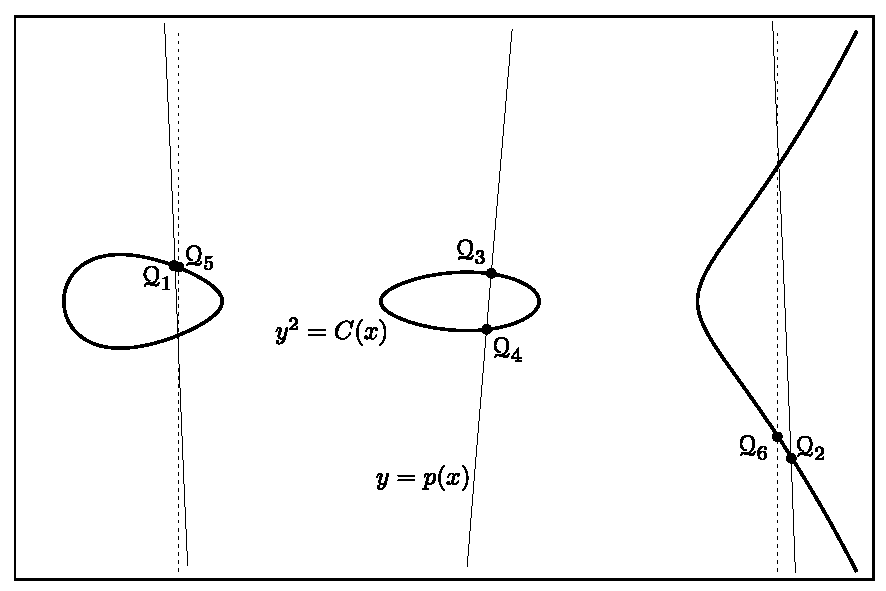
\includegraphics[width=0.9\textwidth]{addition_almost_zero.pdf}

    {\scshape Figure 0a}: Illustrating a limit argument where $\q_3$ is very close to $\bar \q_4$.

    \vspace{1mm}

    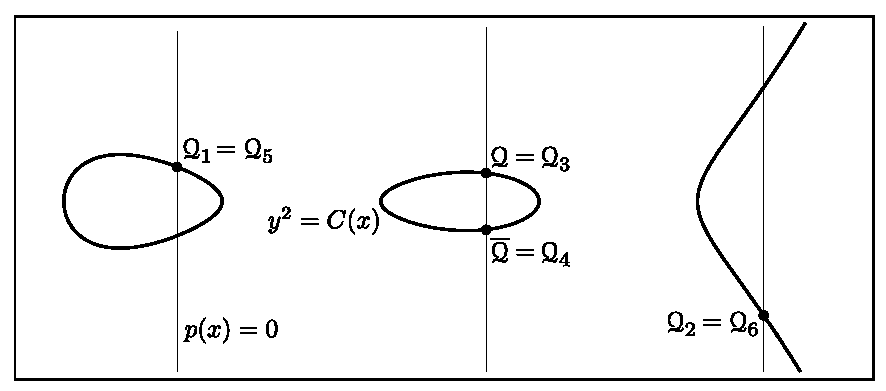
\includegraphics[width=0.9\textwidth]{addition_zero.pdf}

    {\scshape Figure 0b} The addition with zero and justifying $\{ \q , \bar \q \} \sim 0$.
  \end{center}
  \vspace{-1.5mm}
  \fline
\end{figure}

\setcounter{case}{1}
\begin{case}
  {\scshape Tangential:} Let $\q_i\in \enkb, \q_1 = \q_2$, $y_1 \neq 0$ but $x_1$, $x_3$ and $x_4$ are pairwise distinct. We cannot use the Vandermonde matrix in this case because it won't possess maximal rank, consequently being non-invertible. We can however obtain an additional equation by demanding that our polynomial $P(x)$ be tangential to the curve at $\q_1$. This gives
  \begin{align*}
    2 y \frac{dy}{dx} &= 5  x^4 + 4 a x^3 + 3 b x^2 + 2 c x + d \\
    \rlap{\hspace{-37.5mm} and} \frac{dy}{dx} &= 3 p_3 x^2 + 2 p_2 x + p_1
  \end{align*}
  meaning that the system to solve for $\mathbf{p}$ is now $\Vdoub \cdot \mathbf{p} = \ydoub$ with
  \begin{align*}\Vdoub=
    \begin{pmatrix}
      1 & x_1 & x_1^2 & x_1^3\\
      0 & 1 & 2 x_1 & 3 x_1^2\\
      1 & x_3 & x_3^2 & x_3^3\\
      1 & x_4 & x_4^2 & x_4^3\\
    \end{pmatrix}.
  \end{align*}
  The subscript indicates at which points the intersections have higher order.
  Here $\ydoub$ is defined as $\mathbf{y}$ with $y_2$ replaced by $y_2'=\frac{C'(x_1)}{2 y_1}$ where $C'(x)$ is the derivative of $C$ and $2y_1 \neq 0$ because char$(\bar K) \neq 2$ and $y_1\neq 0$. Since $\det(\Vdoub) = (x_4-x_1)^2(x_3-x_1)^2(x_4-x_3)$ this fits neatly into our constraints by being non-zero exactly in the case where $x_1, x_3$ and $x_4$ are pairwise distinct.

\begin{figure}[ht]
  \fline
  \begin{center}
    \vspace{1mm}
    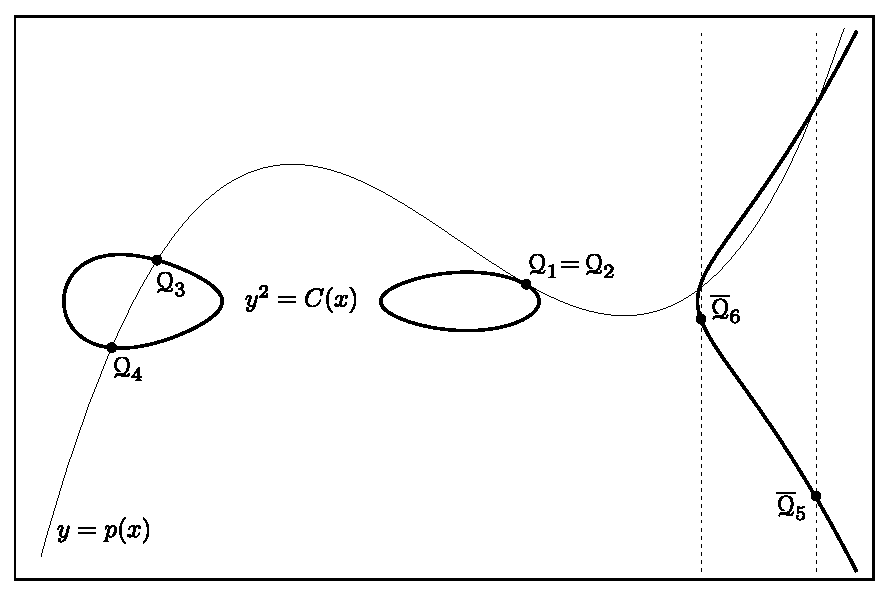
\includegraphics[width=0.9\textwidth]{addition_single_tan.pdf}

    {\scshape Figure 2}: The case of a tangential intersection at $\q_1$.
  \end{center}
  \vspace{-1.5mm}
  \fline
\end{figure}

  Once the polynomial is determined, we note that the $p^2(x)$ shares a tangent with $C(x)$ at $x_1$ on purpose, specifically
  \begin{align*}
    D'(x_1) &= C'(x_1) - 2 P(x_1)p'(x_1)\\
            &= C'(x_1) - 2 y_1 y_2' = 0
  \end{align*}
  so we use Lemma \ref{div} to see that the lefthand side of \eqref{sex} either factors as
  \begin{align} \tag{$*_2$} \begin{split}
    D(x) &= -p_3^2(x-x_1)^2 \prod_{i=3}^6(x-x_i)\\
    \rlap{\hspace{-37mm} or}
    D(x) &= (x-x_1)^2 \prod_{i=3}^5(x-x_i).
  \end{split} \end{align}
  Now step two will be entirely identical to that of the general case and we can again solve \eqref{dagger2} or \eqref{dagger} for $x_5$ or $x_5$ and $x_6$.
\end{case}

\begin{figure}[ht]
  \fline
  \begin{center}
    \vspace{1mm}
    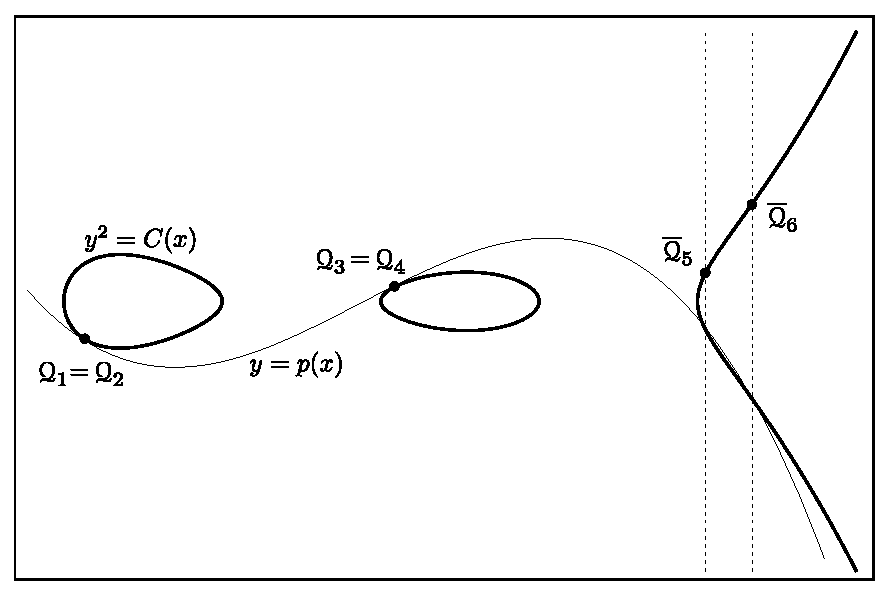
\includegraphics[width=0.9\textwidth]{addition_double_tan.pdf}

    {\scshape Figure 3}: Two tangential intersection at $\q_1$ and $\q_3$ respectively.
  \end{center}
  \vspace{-1.5mm}
  \fline
\end{figure}

\begin{case}
  {\scshape Double Tangential:} Let $\q_i \in \enkb$, $\q_1 = \q_2$ and $\q_3 = \q_4$ but $x_1 \neq x_3$ and $\q_i \neq \bar \q_i$ meaning that neither $y_1$ nor $y_3$ will be zero. As before, we lack equations for our linear system, requiring the use of a second tangential constraint. Replace the fourth row of $\Vdoub$ and $\ydoub$ exactly like we did for the second one: $y_4'=\frac{C'(x_3)}{2 y_3}$ and
  \begin{align*}\Vddoub=
    \begin{pmatrix}
      1 & x_1 & x_1^2 & x_1^3\\
      0 & 1 & 2 x_1 & 3 x_1^2\\
      1 & x_3 & x_3^2 & x_3^3\\
      0 & 1 & 2 x_3 & 3 x_3^2\\
    \end{pmatrix}.
  \end{align*}

  Now $\det(\Vddoub)=(x_3-x_1)^4$ and this is again different from zero precisely whenever $x_3 \neq x_1$, so as before solve $\Vddoub \cdot \mathbf{p} = \yddoub$ for $\mathbf{p}$, then note that $D(x)$ has double zeroes at $x_1$ and $x_3$ by the same argument as in case 2.
  By Lemma \ref{div} we know that \eqref{sex} has a factor $(x-x_1)^2(x-x_3)^2$ so we use
  \begin{align} \tag{$*_3$} \begin{split}
    D(x) &= -p_3^2(x-x_1)^2 (x-x_3)^2 (x-x_5)(x-x_6)\\
    \rlap{\hspace{-25mm} or}
    D(x) &= (x-x_1)^2 (x-x_3)^2 (x-x_5).
  \end{split} \end{align}
  and the procedure of case 1 with $x_2 = x_1$ and $x_4 = x_3$ to solve \eqref{dagger} or \eqref{dagger2}.
\end{case}


\begin{case}
  {\scshape Triple Point:} Let $\q_i \in \enkb , \q_1=\q_2=\q_3$ but $x_1 \neq x_4$ and $y_1 \neq 0$. We can thus see this as a third-order intersection and demand that the curve and the polynomial share a second-order derivative at $\q_1$:
  \begin{align*}\Vtri=
      \begin{pmatrix}
      1 & x_1 & x_1^2 & x_1^3\\
      0 & 1 & 2 x_1 & 3 x_1^2\\
      0 & 0 & 2 & 6x_1\\
      1 & x_4 & x_4^2 & x_4^3\\
    \end{pmatrix}.
  \end{align*}
  Here $\det(\Vtri)=2(x_4-x_1)^3$ and with this, define $\ytri$ by taking $\ydoub$ and replacing the third coordinate by $y_3'' = \frac{C''(x_1)}{2y_1}-\frac{(C'(x_1))^2}{4y_1^3}$ where $C''(x)$ is the second-order derivative of $C$.

\begin{figure}[ht]
  \fline
  \begin{center}
    \vspace{1mm}
    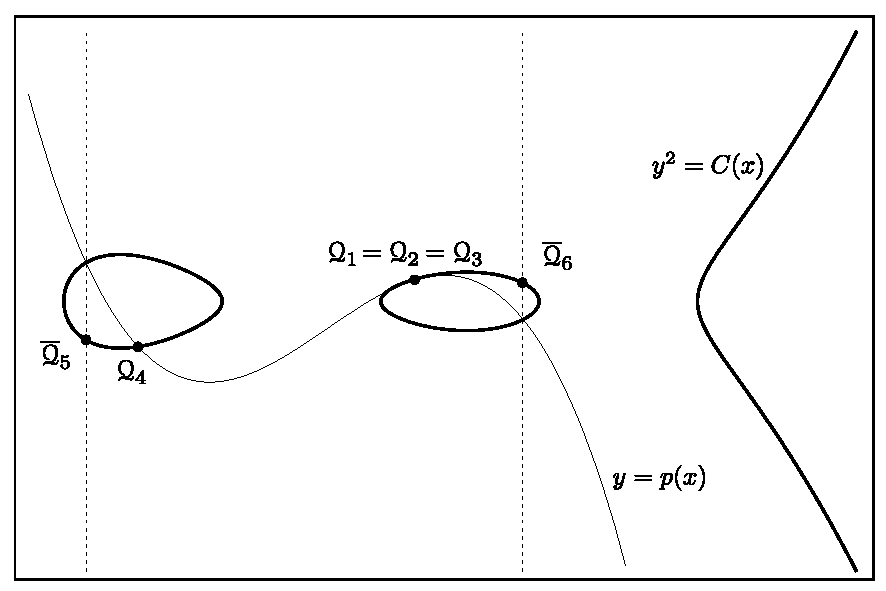
\includegraphics[width=0.9\textwidth]{addition_triple.pdf}

    {\scshape Figure 4}: An intersection of order three at $\q_1$.
  \end{center}
  \vspace{-1.5mm}
  \fline
\end{figure}

  Apply Lemma \ref{div} as in case 2, only this time we also have
  \begin{align*}
    D''(x_1) &= C''(x_1) - 2 P(x_1)p''(x_1) - 2 (p'(x_1))^2\\
             &= C''(x_1) - 2 y_1 y_3''- 2(y_2')^2 = 0
  \end{align*}
  as can be checked by glancing at the definition of $y_3''$. With \eqref{sex} factoring as
  \begin{align} \tag{$*_4$} \begin{split}
    D(x) &= -p_3^2(x-x_1)^3 \prod_{i=4}^6(x-x_i) \\
    \rlap{\hspace{-37mm} or}
    D(x) &= (x-x_1)^3 \prod_{i=4}^5(x-x_i),
  \end{split} \end{align}
  this allows us to continue with one of the second steps of case 1 to find $\P_3$.
\end{case}


\begin{case}
  {\scshape Quadruple Point:} Given the situation where $\q_i = \q_1 \in \enkb$ for every $i$ with $y_1 \neq 0$, we use
  \begin{align*}\Vquad &=
    \begin{pmatrix}
      1 & x_1 & x_1^2 & x_1^3\\
      0 & 1 & 2 x_1 & 3 x_1^2\\
      0 & 0 & 2 & 6x_1\\
      0 & 0 & 0 & 6\\
    \end{pmatrix}
  \end{align*}
  which is invertible in all fields but those of characteristic 2 and 3.

\begin{figure}[ht!]
  \fline
  \begin{center}
    \vspace{1mm}
    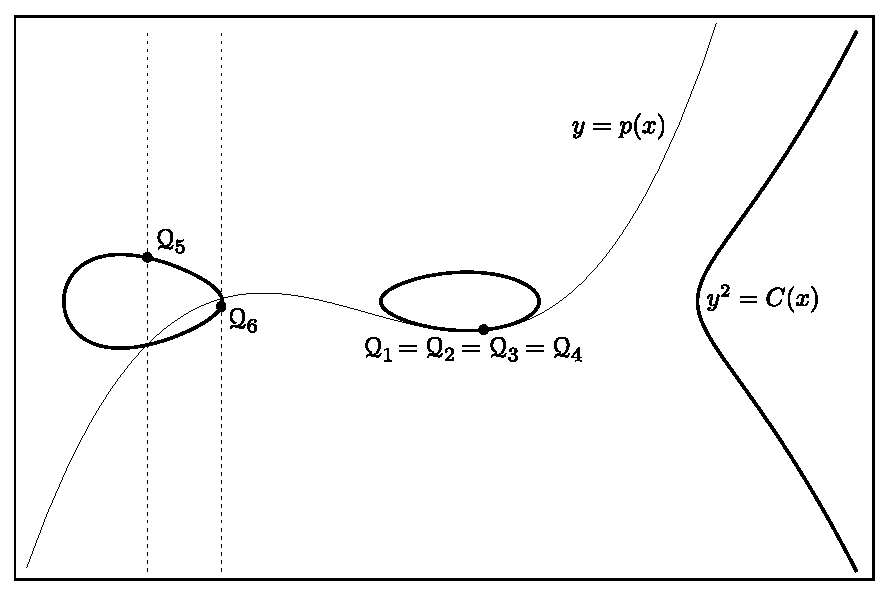
\includegraphics[width=0.9\textwidth]{addition_quadruple.pdf}

    {\scshape Figure 5}: An intersection of order four at $\q_1$.
  \end{center}
  \vspace{-1.5mm}
  \fline
\end{figure}

  Here $\yquad$ is the same as $\ytri$ except for the last coordinate which should read
  \begin{align*}
    y_4''' = \frac{C'''(x_1)}{2y_1}-\frac{3C'(x_1)C''(x_1)}{4y_1^3}+\frac{3(C'(x_1))^3}{8y_1^5}
  \end{align*}
  where $C'''(x)$ is the third-order derivative of $C$. Once more, we solve the linear system $\Vquad \cdot \mathbf{p}=\yquad$. In addition to $D^{(i)}(x_1)=0$, $i=0,..,2$ we have
  \begin{align*}
    D'''(x_1) = C'''(x_1) - 2 y_1 y_4''' - 6 y_2' y_3'' = 0
  \end{align*}
  \vspace{-6mm}
  \begin{align} \tag{$*_5$} \begin{split}
    \rlap{\hspace{-32.5mm} so either} D(x) &= -p_3^2(x-x_1)^4(x-x_5)(x-x_6) \\
    \rlap{\hspace{-32.5mm} or}  D(x) &= (x-x_1)^4(x-x_5)
  \end{split} \end{align}
  which we subsequently use to solve \eqref{dagger} or \eqref{dagger2} and we're done.
\end{case}

\begin{center}
$\sim$
\end{center}

\textbf{Finally}, as noted in Remark \ref{rem}, \eqref{extend} we have yet to extend our definition from $\enkb$ to $\ekb$. Observe that this is relevant only for cases number two and four where we now consider $\q_4 = \infty$ as we did in {\scshape Step $1'$} of the general case. As an analogue to this, the relevant matrices $\tilde V_1$ and $\tilde V_{11}$ will be the upper-left $3 \times 3$ sub-matrices of their $\enkb$-counterparts $V_1$ and $V_{11}$.

In both cases we obtain a linear system of the form $\tilde V_{\ast} \cdot \mathbf{p} = \tilde \mathbf{y}_{\ast}$ for a three-element vector $\mathbf{p}$ and the vectors $\tilde \mathbf{y}_{1}$ and $\tilde \mathbf{y}_{11}$ are defined like their 4-element counterparts $\mathbf{y}_{1}$ and $\mathbf{y}_{11}$ with the last coordinate omitted.

Both matrices $\tilde V_{\ast}$ are invertible and we therefore get a unique polynomial $P(x)$ wich we use to solve \eqref{daggerp}, obtaining $x_5$, $x_6$, $y_5=P(x_5)$ and $y_6=P(x_6)$ in $\bar K$ and we define $\{ \q_1 , \q_2\}+\{ \q_3 , \infty \} = \{ \bar \q_5 , \bar \q_6 \} = \{(x_5,-y_5),(x_6,-y_6)\}$.

The counterparts to ($*_2$) and ($*_4$) in these cases are
\begin{align*}
  \tag{$*_2'$} D(x) &= (x-x_1)^2(x-x_3)(x-x_5)(x-x_6)\\
  \rlap{\hspace{-29.3mm} and}
  \tag{$*_4'$} D(x) &= (x-x_1)^3(x-x_5)(x-x_6)
\end{align*}

\subsection{Well-Definedness of the Addition Law}

To check whether our addition is well defined on $\J$ in each of the cases, we have to consider the permutation of point-components $\q_i$ under the equivalence relation from Definition \ref{defj}. Furthermore, to claim that all possible cases are all covered, it is necessary to check the permutations under \eqref{switch}. Both cases can be combined into a single one by the following statement:

\begin{lemma}
In each given definition of ``$+$'', the result $\{ \q_5, \q_6 \}$ is invariant under the interchange of $\q_i$ and $\q_j$ for any $i,j \in \{ 1,..,4 \}$.

\begin{proof}
  Case 0 was done at \eqref{zero}.
  In cases 1--5, interchanging $x_i$ with $x_j$ and $y_i$ with $y_j$ in our linear systems $V_{\ast} \cdot \mathbf{p} = \mathbf{y}_{\ast}$ has the effect of permuting rows of $V_{\ast}$ and $\mathbf{y}_{\ast}$ and relabeling $(x_k,y_k)$ whenever $\q_k$ was equal to $\q_i$ or $\q_j$.

  Consequently the resulting $P(x)$ doesn't change, so neither do any of the terms $T_{\ast}$. The three dagger equations remain unchanged as well, as can easily be checked at \eqref{dagger}, \eqref{dagger2} and \eqref{daggerp} which are invariant under the interchange of $x_i$ and $x_j$. Finally, the version of Step 2 we fall into remains the same, since it is only imposed by the distinction of $p_3$ being zero or not. 
\end{proof}
\end{lemma}

\subsection{Summary and Conclusions}

For the convenience of the reader we attempt to summarize our approach and give some preliminary implications. First, whenever we refer to $\q_i$ in $\ekb$, $\q_i = (x_i, y_i)$ for $i = 1,..,6$, from now on it is implicitly understood to be in the context of the sum
\begin{align*}
  \{\q_1, \q_2 \} +\{ \q_3 , \q_4 \} = \{\bar \q_5 , \bar \q_6\}
\end{align*}
where our goal was to define $\q_5$ and $\q_6$. We started with $x_1, x_2, x_3, x_4$ all finite and different and used the graph of a cubic polynomial $P(x)$ which may however degenerate into a quadratic, linear or even constant one. The two new intersections of the graph of the polynomial with the curve would then determine the result of our sum. For this, we used the polynomial $D(x)=C(x)-(P(x))^2$ (see Remark \ref{remD}). If there is only one new intersection, we call the other one $\infty$. There is at least one new intersection as $D(x)$ had degree six or five which can have no less than five roots in $\bar K$.

As a first generalization we allowed for $\q_4 = \infty$ with $x_1, x_2, x_3$ still all finite and different. In that case, $D(x)$ has degree five, so $x_5$, $x_6$ have to be finite.

This completed case 1 ``all $x_i$ different'' because \eqref{switch} allowed interchanging $\q_4$ with $\q_1, \q_2$ or $\q_3$. This symmetry was consistent with the addition rule so far and it furthermore allowed us to say that, if $\q_i = \bar \q_j$ for $i \neq j$, $\q_i \neq \q_j$, then we are in the zero case. We used this to write the complete list of cases, considering four cases of $x_1,..,x_4$ finite but not different. We completed each case with $x_1,..,x_3$ finite but $x_4 = \infty$ as we did for case 1.

We can extend the distinction ``$\q_i \neq \bar \q_j$'' between zero and non-zero cases.

\begin{lemma}\label{atmost1}
  Provided we are not in case 0, then $\q_i \neq \bar \q_j$ for $i \neq j$, $\q_i \neq \q_j$ is not only true for $i,j = 1,..,4$ but for $i,j = 1,..,6$ as well.

  \begin{proof}
    All points $\q_i = (x_i,y_i) \neq \infty$ lie on the graph of $P$, so no two points can have the same $x$-coordinate but different $y$-coordinates.
    %$y_i = P(x_i)$, so if two points have the same $x$-coordinate and opposing $y$-coordinates, $y_i$ must equal 0. This means $\q_i = \q_j$, which contradicts the premise.
  \end{proof}

  %Provided we are not in case 0, then at most one of the six point-components $\q_1,..,\q_6$ may equal $\infty$. This is easy to check as in every case, either all $\q_1, \q_2, \q_3, \q_4$ are finite so only one of $\q_5, \q_6$ may be infinite, or $\q_4 = \infty$ in which case both $\q_5$ and $\q_6$ are finite as mentioned above.

  A very useful special case of ``$\q_i \neq \bar \q_j$'' is that no more that one of the six components $\q_1,.., \q_6$ may equal $\infty$ in non-zero cases.
\end{lemma}

% \vspace{-3mm}
% \begin{center}
% $\sim$
% \end{center}
% \vspace{-2mm}

The symmetry we defined at \eqref{switch} will turn out to be a provable property, but we can already broaden it in the next Lemma.

\begin{lemma}\label{symall}
  The symmetry imposed on the sum in $\q_1, .., \q_4$ now extends to symmetry in $\q_1, .., \q_6$. For instance, once we explicitely derive the sum $\{\q_1, \q_2 \} +\{ \q_3 , \q_4 \} = \{\bar \q_5 , \bar \q_6\}$, we know that $\{\q_5, \q_2 \} +\{ \q_3 , \q_4 \} = \{\bar \q_1 , \bar \q_6\}$.
\end{lemma}

To see why this is obvious, we first summarize the various $D(x)$ we derived at ($*_1$) through ($*_5$) and ($*_1'$), ($*_2'$) and ($*_4'$) for cases 1--5 and give the simplest general expression possible.

\begin{remark}\label{remD}
  In every non-zero case we have a polynomial $P$ whose graph we let intersect the curve such that the new intersections give $\q_5$ and $\q_6$ where they are finite. This is done by finding $x_5$ and $x_6$ if they exist, which in turn was done by solving $D(x) = 0$ where we defined $D(x) = C(x) - (P(x))^2$.

  In all non-zero cases we manually derived the expression for the various $D(x)$ at ($*_i$) and ($*_i'$) for cases 1--5, which all come down to
  \begin{align*}
    D(x) &= -p_3^2\prod_{i=1}^6(x-x_i)
  \end{align*}
  if $p_3 \neq 0$. If $p_3 = 0$ and therefore $\q_j = \infty$ for exactly one $j \in \{1,..,6\}$ then
  \begin{align*}
    D(x) &=  \prod_{\substack{i=1\\i \neq j}}^6(x-x_i).
  \end{align*}
  Remember that at most one of the $\q_i$ can be $\infty$, covering all non-zero cases.

  For later use we can even write the more compact product
  \begin{align*}
    D(x) &= \delta \prod_{\q} \big(x-x(\q)\big)^{e(\q)}
  \end{align*}
  taken over all $\q  \in \enkb$ where $e(\q)$ is the number among $\q_1,..,\q_6$ that equal $\q = (x(\q), y(\q))$. This works because by Lemma \ref{atmost1}, if $x_i = x_j$ for $i \neq j$, then $\q_i = \q_j$.
\end{remark}

\emph{Proof of Lemma \ref{symall}.}
  Both expressions above remain unchanged under permutation on the $x_i$. And since $\q_i = (x_i, y_i)$ with $y_i = P(x_i)$, we're done.

  Last but not least, this Lemma remains universally valid, as the property can be checked for the zero case as well through a quick glance at \eqref{zero}.\hfill \qed



%\textit{For the convenience (sanity?) of the reader and to simplify the proofs of Section 3 the sheer number of case-distinctions and sub-cases lend themself simplification by reviewing and summarizing our findings, definitions and their implications.}


% \begin{remark}
%   Looking back at the complete list of cases, we simplified things twofold. First, \eqref{switch} implied that exchanging $\q_i$ and $\q_j$ for $i,j \in \{1,..,4\}$ can't change the sum. Second, we isolated the zero case in order to state that in any other case the situation $\q_i = \bar \q_j$ for $i \neq j$, $i, j = 1,..,4$ never occurs, in other words in the non-zero case we have $\q_i = \q_j \iff x_i = x_j$.

%   % through $\{\q_1, \q_2 \} +\{ \q_3 , \q_4 \} = \{\bar \q_5 , \bar \q_6\}$

%   Now after obtaining $\q_5$ and $\q_6$ we would very much like for the above two properties to be true for $i,j = 1,..,6$.

%   Fortunately they are: ...

%   % Now, by construction of the sum in all non-zero cases it is easy to check that the same properties hold for the whole set $\{ \q_i \mid i = 1,..,6 \}$ for a given sum.

%   % The polynomial $P(x)$ passes through all those $\q_i$ that are in $\enkb$. This implies that if $\q_i = \bar \q_j$ we must have $-y_i = y_j = P(x_j) = P(x_i) = y_i$ so $y_i = 0$ in char$(K) \neq 2$ i.e. $\bar \q_i =\q_j = \q_i$. This is helpful for the next proof.
% \end{remark}

%------------------------------------------------------------------------------
\newpage
%------------------------------------------------------------------------------

\section{Rational Functions on Hyperelliptics}

The goal of this chapter is to look at rational functions on the hyperelliptic curve $y^2 = C(x)$ and to define a notion of the order of a function in a point on the curve. We then give some basic properties for this order function before we introduce divisors and proceed to look at functions with a specified number of poles at $\infty$ as a preparation for the proof of associativity on $\J$.

\subsection{Function Field and Order of Rational Functions}

\begin{defin}
  Define the ring of rational functions on the curve as
  \begin{align*}
    \F = \bigslant{K(x)[y]}{\big(y^2-C(x)\big)}.
  \end{align*}
  As $y^2-C(x)$ is irreducible in $K(x)[y]$, $\F$ is a field
  % want me to write why?
  and $\F = K(x) + K(x) y$, so write elements $f \in \F$ as $f = g + hy$ where $g,h \in K(x)$. Define $\bar f = g - hy$.

  We will occasionally write things like $K[x,y] \subset \F$ but this is always implicitly understood to be in conjunction with $y^2=C(x)$.
\end{defin}

\vspace{3mm}

\textbf{Reminders}: A formal Laurent series written $\tau = \gamma t^e (1 + \cdots)\in K (\! (t)\! )$ with $\gamma \in K^*$, $e \in \mathds{Z}$ has a a unique inverse $\tau^{-1} = \gamma^{-1} t^{-e} (1 + \cdots) \in K (\! (t)\! )$.

From now on we will use an ellipsis to denote any terms of ascending order everywhere where we are not interested in the specifics.

If char$(K) \neq 2$ and $\tau$ is a series of the form $\tau = 1 + \sum_{i = 1}^{\infty} a_i t^i$ then it has a unique square root of the form $\sigma = 1+\sum_{i = 1}^{\infty} b_i t^i$ in $\bar K (\! (t)\! )$ meaning $\sigma^2 = \tau$. Write $\sigma = \sqrt \tau = 1 + \cdots$.

\vspace{-3mm}
\begin{center}
$\sim$
\end{center}

In order to define the order of a function $f$ in a point $\q$, $\ordq (f) \in \mathds{Z}$ for $f \in \F^*$ and $\q \in \ekb$ we first construct a $K$-homomorphism
\begin{align*}
  \lp: \F \rightarrow \bar K (\! (t)\! )
\end{align*}
% with the intent of defining $\ordq(f) = \ord \lp (f)$.
Because $C\big(\lpx\big)=\big(\lpy\big)^2$ has to be fulfilled, we decide on $\lpx$ and deduce $\lpy$. For this, we distinguish between three cases for $\q \in \ekb$.

\newpage

\begin{defin}\label{def-lambda}
  \begin{enumerate}[1.]
    \item Let $\q =(x_0,y_0) \in \enkb$ with $y_0 \neq 0$ and consequently $C(x_0)\neq 0$.

    Define $\lpx = x_0 + t$. Now
    \begin{align*}
      C(\lpx) &= C(x_0+t)\\
              &= C(x_0)+ \cdots + t^5\\
              &= C(x_0)(1 + \cdots)\\ % \text{ since } C(x_0) = y_0^2\neq 0\\
              &= y_0^2 \tau_1 \text{\hspace{5mm} with } \tau_1 \in K (\! (t)\! ).
    \end{align*}
    Define $\lpy = y_0 \sqrt{\tau_1}$.

    \item Let $\q =(x_0,y_0) \in \enkb$ with $y_0 = 0$. Points with this property are called ``Weierstrass Points'' and as $C(x_0)=0$ there are at most five of them. Write $C(x)=\prod_{i=1}^5 (x-\alpha_i)$ for $\alpha_i \in \bar K$ and for instance $\alpha_1 = x_0$.

    Define $\lpx = x_0 + t^2$. Now
    \begin{align*}
      C(\lpx) &= t^2 \prod_{i=2}^5 (x_0 -\alpha_i + t^2) \\
              &= \mu t^2 (1 + \cdots)
    \end{align*}
    with $\mu \in \bar K$ being $\mu = \prod_{i=2}^5 (x_0 - \alpha_i) = C'(x_0)$ which is non-zero because our curve is non-singular. Write therefore $C(\lpx) = \mu t^2 \tau_2$ with $\tau_2$ of the form $1 + \cdots$ and define $\lpy = \nu t \sqrt{\tau_2}$ with $\nu^2 = \mu$, $\nu \in  \bar K$.

    Note that we may choose one out of two square roots for $\nu$ so whichever we take we demand that we stay consistent in our choice for now. It will however turn out that this choice bears no effect on definition \ref{def-ord}.

    \item Let $\q = \infty$. Define $\lpx = t^{-2}$. It follows that
    \begin{align*}
      C(\lpx) &= t^{-10} + at^{-8} + bt^{-6}
                        + ct^{-4}    + dt^{-2} + e\\
                       &= t^{-10} \sqrt{\tau_3}
    \end{align*}
    so define $\lpy = t^{-5} \sqrt{\tau_3}$.
  \end{enumerate}
\end{defin}


\vspace{-3mm}
\fline
\vspace{-3mm}
\begin{defin}\label{def-ord}
   For $\q \in \ekb$ and $f \in \F^*$ define $\ordq (f) = \ord \lp (f)$.
\end{defin}
\vspace{-5.5mm}
\fline

% \begin{center}
% $\sim$
% \end{center}
% \vspace{0.6mm}

\begin{lemma}\label{one}
  Let $f \in K[x,y] \subset \F$, $f \neq 0$ and $\q \in \enkb$, $\q = (x_0,y_0)$. Then
  \begin{enumerate}[(a)]\parskip 1mm
    \item ord$_{\q} f \geq 0$ and
    \item if $f(\q) = 0$ then ord$_{\q} f \geq 1$.
  \end{enumerate}\parskip 3mm
  \begin{proof}\hfill
    \begin{enumerate}[(a)]\parskip 1mm
      \item Because $\q \in \enkb$ we have $\lpx$, $\lpy \in \bar K[[t]]$ so with $f \in K[x,y]$ we have $\ordq (f) \in \mathds{N} \cup \{0\}$.
      \item Write $f = A(x,y)$, $A(X,Y) \in K[X,Y]$. First, let $y_0 \neq 0$.
      \begin{align*}
        \ordq f &= \ord A(\lpx, \lpy)\\
        &= \ord A(x_0 + t, y_0 \sqrt \tau_1).
      \end{align*}
      But $A(x_0 + t, y_0 \sqrt \tau_1)=\sum_{i=0}^{\infty} a_i t^i$ so with $t=0$ we get $A(x_0, y_0)=a_0$ but the former is $f(\q)$ which is $0$, so $a_0 = 0$ and the claim follows.

      If $y_0 = 0$ we would have $\ordq f = \ord A(x_0 + t^2, \nu t \sqrt \tau_2)$ instead. But like before, this means $0 = f(\q) = A(x_0, 0) = a_0$ so again $\ordq (f) \geq 1$.
    \end{enumerate}\parskip 3mm
  \end{proof}
\end{lemma}

\begin{lemma}\label{two}
  Let $f \in K(x) \subset \F$, $f \neq 0$, $\q \in \ekb$. Then
  \begin{enumerate}[(a)]\parskip 1mm
    \item $\ordq (f) = \ordx f(x)$ if $\q = (x_0,y_0) \in \enkb$ with $y_0 \neq 0$.
    \item $\ordq (f) = 2 \ordx f(x)$ if $\q = (x_0,0) \in \enkb$.
    \item $\ordi (f) = 2 \ordii f(x) = 2 \ordn f(\frac 1 x)$.
  \end{enumerate}\parskip 3mm
  \textbf{Note} that the right-hand sides of the equalities refer to the usual definition of the order of a rational function in a point $x_0 \in \bar K \cup \{ \infty \}$.% We will not always write the function argument.
  \begin{proof}
    Take $f \in K[x]$ and define $e = \ordx f \in \mathds{N}$ so $f(x) = (x-x_0)^e g(x)$ with $g \in \bar K[x]$ and $g(x_0)\neq 0$.
    \begin{enumerate}[(a)]
      \item If $\q =(x_0,y_0)$, $y_0 \neq 0$ then $\lp (f) = f(x_0 + t) = t^e g(x_0 + t)$ and so $\ord \lp (f) = e$ because $g(x_0 + t) = g(x_0) + \cdots$ with $g(x_0) \neq 0$.

      \item Here $\lp (f) = f(x_0 + t^2) = t^{2e} g(x_0 + t^2)$ and again $g(x_0 + t^2) = g(x_0) + \cdots$ so $\ord \lp (f) = 2e$.

      \item For $\q = \infty$ we have $\lp (f) = f(t^{-2}) = \kappa t^{-2d}+ \cdots$ with $\kappa \neq 0$ if $d = \deg f$ so $\ordn f(\frac 1 x ) = -d$ and so $\ord \lp (f) = 2 \ordn f(\frac 1 x )$.
    \end{enumerate}
    Generally, if $f \in K(x)$ we can write $f = \frac r q$ for $r, q \in K[x]$ and apply $\ordx f = \ordx r - \ordx q$ in order to use the above on $r$ and $q$.
  \end{proof}
\end{lemma}

\begin{lemma}\label{three}
  For $f \in \F^*$ and $\q \in \ekb$ the order satisfies $\ordq(\bar f) = \ordbq (f)$
  \begin{proof} Split into three possible cases:
    \begin{enumerate}[1.]
      \item For $\q \in \enkb$ with $y_0 \neq 0$ we've got $\lpx = x_0 + t$ and $\lpy = y_0 \sqrt \tau_1$. Therefore $\lpbx = x_0 + t = \lp (\bar x)$ and $\lpby = - y_0 \sqrt \tau_1 = \lp (\bar y)$ so
      \begin{align*}
        \lpb (f(x,y)) &= f(\lpbx , \lpby ) \\
                      &= \lp (f(\bar x, \bar y)) \\
                      &= \lp (\bar f (x,y)).
      \end{align*}

      \item If $\q \in \enkb$ with $y_0 = 0$ then $\bar \q = \q$. Write $f(x) = g(x) + h(x)y$, so
      \begin{align*}
        \lp (\bar f) &= g(x_0 + t^2) - h(x_0 + t^2) \nu t \sqrt{\tau_2}.
      \end{align*}
      Calling this $l(t) = \lp (\bar f)$ and looking at the construction of $\lp$ we see that $\tau_2$ sports only even powers of $t$ so we see above that $l(-t) = \lp (f)$. As interchanging $t$ with $-t$ doesn't change the order, we're done.

      \item For $\q = \infty$, $\tau_3 = 1 + a t^2 + b t^4 + c t^6 + d t^8 + e t^{10}$ features only even powers as well, so again $l(-t) = \lp (f)$ for $l(t) = \lp (\bar f) = g(t^{-2}) - h(t^{-2}) t^{-5} \sqrt{\tau_3}$. Finally, $\lp (f)$ is equal to $\lpb (f)$ since $\infty = \bar \infty$. Again $\ord l(t) = \ord l(-t)$.
    \end{enumerate}
  \end{proof}
\end{lemma}

\begin{remark}
  We now see why the choice of the square root in definition \ref{def-lambda} has no effect on $\ordq f$. If $\lp'$ were to correspond to the other choice, we would have $\lp'(x) = \lp(x)$ and $\lp'(y) = -\lp(y)$, so $\lp'(f) = \lp (\bar f)$. As this was under item 2 where $y_0 = 0$, meaning $\bar \q = \q$, we have $\ord \lp (\bar f) = \ord \lp(f)$.
\end{remark}

\begin{lemma}\label{sform}
  %(Summenformel)
  If $f \in \F^*$ then the set $\big \{ \q \in \ekb \ \big | \ \ordq f \neq 0 \big \}$ is finite and
  \begin{align*}
    \sum_{\q \in \ekb} \ordq f = 0.
  \end{align*}
  \begin{proof}
    First take $f \in K[x,y]$, $f \neq 0$ and let $\q = (x_0,y_0) \in \enkb$, $y_0 \neq 0$, with $\ordq f \neq 0$. By Lemma \ref{one} (a) we know that $\ordq f \geq 1$. It follows that $\ordq (f \bar f) = \ordq f + \ordq \bar f \geq 1$. Now since $f = g + h y$, $f \bar f = g^2 - h^2 C(x)$ which lies in $K[x]$, so by Lemma \ref{two} we have $\ordx (f \bar f) = \ordq (f \bar f) \geq 1$. But there are only finitely many such $x_0$ and so only finitely many such $y_0 = \pm \sqrt{C(x_0)}$.

    If $f \in K(x,y)$, $f = \frac r q$, $r, q \in K[x,y]$ then $\ordx f = \ordx r - \ordx q$, and again only finitely many $x_0$ exist for which this differs from zero.

    For the second claim, give our sum the name
    \begin{align*}
      s(f) &= \sum_{\q \in \ekb} \ordq f
    \end{align*}
    and note that $s(f) = s(\bar f)$ due to Lemma \ref{three} and the fact that we take the sum over all $\q$. Because $\ordq (f \bar f ) = \ordq (f) + \ordq ( \bar f )$ we can see that
    \begin{align*}
      s(f \bar f) &= s(f) + s(\bar f) = 2 s(f).
    \end{align*}
    But because $f \bar f \in K(x)$ we can use Lemma \ref{two} to write this out as
    \begin{align*}
      2s(f) &= \sum_{\q \in \ekb} \ordq f \bar f\\
            &=2 \mathop{\sum_{x_0 \neq \infty}}_{C(x_0) \neq 0} \ordx f \bar f 
            + 2 \mathop{\sum_{x_0 \neq \infty}}_{C(x_0) = 0} \ordx f \bar f 
            + 2 \sum_{x_0 = \infty} \ordx f \bar f\\
            %
            &=2 \sum_{x_0 \in \bar K \cup \{ \infty \}} \ordx f \bar f.
    \end{align*}
    %Here $\alpha_i$ are the points on which $C(x)$ vanishes and since
    \begin{align*}
    \rlap{\hspace{-45mm} Since}
      \sum_{x_0 \in \bar K \cup \{ \infty \}} \ordx g = 0
    \end{align*}
    for any $g \in K(x)$ we have $s(f) = 0$ in $\mathds{Z}$.
  \end{proof}
\end{lemma}

% \begin{center}
% $\sim$
% \end{center}

\subsection{Divisors and Lemmas}

\begin{defin}
  The divisor of a function $f \in \F^*$ is the formal sum
  \begin{align*}
    (f) = \sum_{\q \in \ekb} \ordq f \cdot \q
  \end{align*}
  Thanks to Lemma \ref{sform} the sum is finite and the sum of all coefficients is 0.

  Points $\q \in \ekb$ with a positive coefficient in $(f)$ are called zeroes of $f$ while those with a negative coefficient are called poles.
\end{defin}

\begin{lemma}\label{nopol}
  If $f \in \F^*$ has no poles on $\ekb$, i.e. if $\ordq f \geq 0$ for all $\q$, then $f$ is constant.
  \begin{proof}
    With $f = g + hy$, $\ordq f \geq 0$ for every $\q \in \ekb$ we take a look at $f + \bar f = 2g \in K(x)$ and $f \bar f = g^2 - h^2 C \in K(x)$ and observe that by well-known properties of orders
    \begin{align*}
      \ordq (f + \bar f) &\geq \min \{ \ordq f , \ordq \bar f \} \\
          &= \min \{ \ordq f , \ordbq f\} \geq 0.
      \intertext{with Lemma \ref{three} and similarly}
      \ordq (f \bar f) &= \ordq f + \ordbq f \geq 0.
    \end{align*}
    With the help of Lemma \ref{two} we conclude that $\ordx (f + \bar f) \geq 0$ and $\ordx (f \bar f) \geq 0$ respectively.

    But in $\bar K(x)$, a function $q$ with $\ordx q \geq 0$ for every $x_0 \in \bar K \cup \{ \infty \}$ must be constant, so both $f + \bar f$ and $f \bar f$ are constant functions. Since $f$ is a root of $(T-f)(T-\bar f) = T^2 - (f + \bar f)T + f \bar f \in \bar K[T]$, $f$ lies in $\bar K \hspace{0.5mm}$.
  \end{proof}
\end{lemma}

\begin{theorem}\label{satz1} \textit{(Proof in appendix)}
  Let $x$, $y \in K(t)$ be rational functions that fulfill $y^2 = C(x)$. Then $x$ and $y$ are actually constants, i.e. $x$, $y \in K$.
\end{theorem}

\begin{lemma}\label{onepol}
  Suppose $f \in \F^*$ has a pole of order at most one at $\infty$ i.e. $\ordi f \geq -1$ and no pole at any other $\q \in \enkb$. Then $f$ is a constant.

  \begin{proof}
    By Lemma \ref{nopol} we can assume $\ordi f = -1$ and $\ordq f \geq 0$ for every $\q \in \enkb$. Now $f = g+hy$ and $\li (f) = \kappa t^{-1} + \cdots$ with $\kappa \neq 0$ in $\bar K$. Since we are only interested in the order, replace $f$ with $\kappa^{-1} f$ so $\li (f) = t^{-1} + \cdots$.

    Now remember that $\li (x) = t^{-2}$ so $\li (x - f^2) = \alpha t^{-1} + \cdots$, $\alpha \in \bar K$ and finally we have a regular power series $\li (x - f^2 - \alpha f)$ so
    \begin{align*}
      \ordi (x - f^2 - \alpha f) &\geq 0.
    \end{align*}
    Also for any other $\q \in \enkb$ we have
    \begin{align*}
      \ordq (x - f^2 - \alpha f) &\geq \min \{ \ordq (x) , \ordq (f^2) , \ordq f \}
    \end{align*}
    which is non-negative by virtue of the prerequisite on $f$ and $\lpx = x_0 + \cdots$. The previous Lemma now implies $x - f^2 - \alpha f \in \bar K$ so we see $x = f^2 + \alpha f + \beta$ as a polynomial $x = X(f)$ with $X(T) \in \bar K[T] \setminus \bar K$.

    \begin{flalign*}
      \rlap{Do the same thing with}
                && \hspace{11mm}
                  \li (y) = t^{-5}\sqrt \tau_3 &= \hspace{3.9mm} t^{-5} + \cdots &\\
      \rlap{so} &&               \li (y - f^5) &=        \beta_4 t^{-4} + \cdots &\\
      \rlap{and}&& \li (y - f^5 - \beta_4 f^4) &=        \beta_3 t^{-3} + \cdots
    \end{flalign*}
    and so on, so $\li (y - f^5 - \beta_4 f^4 - \beta_3 f^3 - \beta_2 f^2 - \beta_1 f)$ is a power series as well. Again $y = f^5 + \beta_4 f^4 + \beta_3 f^3 + \beta_2 f^2 + \beta_1 f + \beta_0 = Y(f)$ with $Y(T)\in \bar K[T] \setminus \bar K$.    

    Combined we have the polynomial equation $Y(f)^2 - C(X(f)) = 0$ over $\bar K$ whose algebraic closure dictates either $f \in \bar K$ or $Y(T)^2 = C(X(T))$. The latter can't be true by Theorem \ref{satz1} and the former is in contradiction to $\ordi f = -1$.
  \end{proof}
\end{lemma}

\begin{lemma}\label{twopol}
  If $f \in \F^*$ has a pole of order at most two at $\infty$ and $\ordq f \geq 0$ for every $\q \in \enkb$ then $f$ is of the form $f = \alpha + \beta x$ with $\alpha, \beta \in K$.
  \begin{proof}
    Because $\li (f) = \beta t^{-2} + \cdots$ where $\beta \in \bar K$ we have $\li (f - \beta x)= \gamma t^{-1} + \cdots$ and thanks to Lemma \ref{onepol} we know this to imply $f - \beta x = \alpha$.
  \end{proof}
  \textbf{Note} that it is easy to see that in this case $(f) = \a + \bar \a -2 \infty$ for $\a = ( - \frac \alpha \beta , * )$
\end{lemma}

\begin{lemma}\label{threepol}
  If $f \in \F^*$ has a pole of order at most three at $\infty$ and $\ordq f \geq 0$ for every $\q \in \enkb$ then $f$ is of the form $f = \alpha + \beta x$ with $\alpha, \beta \in K$.
  \begin{proof}
    From $\li (f) = \gamma t^{-3} + \cdots$ and $f + \bar f \in K(x)$ we get that the order of the latter must be even by Lemma \ref{two} (c), so $\ordi (f+ \bar f)  \geq -2$. Like $f$, $f + \bar f$, has no poles on $\enkb$ so Lemma \ref{twopol} implies $f + \bar f = \alpha + \beta x$. Writing $f = g + hy$ we therefore see that $g = \frac{\alpha + \beta x}{2}$ and $f - g = hy$. The latter also has a pole of order three at $\infty$ and none on $\enkb$ so we are effectively reduced to studying functions $f$ of the form $f = hy$ for $h \in K(x)$, $h \neq 0$.

    Lemma \ref{twopol} lets us assume $\ordi f = -3$. Now with $f = h y$ we have that $-3 = \ordi h + \ordi y = \ordi h - 5$ so $\ordi h = 2$. Writing $h = \frac r q$ for $r, q \in K[x]$ coprime, this means that $q$ cannot be constant. Use this to pick a $\xi \in \bar K$ with $q(\xi) = 0$, implying $r(\xi) \neq 0$ by coprimality.

    Pick a point $\r = (\xi, \eta)$ in $\enkb$. If $C(\xi) \neq 0$ then $\text{ord}_\r \hspace{0.5mm} y = 0$ and $\text{ord}_\r \hspace{0.5mm} q \geq 1$ from which we deduce $\text{ord}_\r \hspace{0.4mm} f = \text{ord}_\r \hspace{0.4mm} \frac y q \leq -1$, a contradiction. In case $\xi$ is a Weierstrass Point, $C(\xi) = 0$ then $\text{ord}_\r \hspace{0.5mm} y = 1$ and $\text{ord}_\r \hspace{0.5mm} q \geq 2$ and so we get the same contradiction. This finishes the proof.
  \end{proof}
\end{lemma}

\begin{lemma}\label{fourpoles}
  If $f \in \F^*$ has a pole of order at most four at $\infty$ and $\ordq f \geq 0$ for every $\q \in \enkb$ then $f$ is of the form $f = \alpha + \beta x + \gamma x^2$ with $\alpha, \beta, \gamma \in K$.
  \begin{proof}
    With $\li (f) = \gamma t^{-4} + \cdots$ we know that $\li (f - \gamma x^2) = \delta t^{-3} + \cdots$ and we use the previous Lemma to see that $f - \gamma x^2 = \alpha + \beta x$.
  \end{proof}
\end{lemma}

%------------------------------------------------------------------------------
\newpage
%------------------------------------------------------------------------------

\section{Associativity}

We return to the context of the sum defined in Chapter \ref{ch1}. Suppose we have $\q_i \in \ekb$, $i=1,..,6$ that fulfill
\begin{align*}
  \{ \q_1 , \q_2\}+\{\q_3 , \q_4\} = \{\bar \q_5 , \bar \q_6 \}.
\end{align*}
If we are in a non-zero case, then we had the graph of a polynomial $P$ passing through all $\q_i \neq \infty$, $i = 1,..,6$. Remember that then, by Lemma \ref{atmost1}, at most one of the $\q_i$ can be $\infty$. We defined $D(x) = C(x) - (P(x))^2$.
%Remember that by Lemma \ref{atmost1} xxx nee!! , if $\q_j = \infty$ for at most one $j \in \{1,..,6\}$, then we are in one of the non-zero cases of the addition law. In such a case, we had the graph of a polynomial $P$ passing through all $\q_i \neq \infty$. We defined $D(x) = C(x) - (P(x))^2$.
\begin{lemma}\label{mult}
  If the sum falls into one of the cases 1--5, pick any $\q_k \neq \infty$ for $k = 1,..,6$, so $\q_k = (x_k, y_k) \in \enkb$. Now it can be said that $\q_k$ occurs exactly $e_k$ times in the expression of the sum, $e_k$ being between
  1 and 6. %\footnotemark[1]
  Then\vspace{-3mm}
  \begin{align*}
    \text{ord}_{x=x_k}\hspace{0.4mm} D(x) = e_k.
  \end{align*}
  % This is of course equivalent to stating $\text{ord}_{x=x_k}\hspace{0.4mm} D(x) = e_k$ which is also the order of the intersection of $P(x)$ and the curve at $\q_k$.% The choice of $k$ does not matter.
  \begin{proof} With  Remark \ref{remD} we know $D(x) = (x - x_k)^{e_k} g(x)$ with $g_k(x_k) \neq 0$.
  \end{proof}
  %Small remark: Any $\q$ can actually only occur four times in the expression of the sum as we would otherwise find ourself in the zero case.
\end{lemma}

%\footnotetext[1]{It can actually be only between 1 and 4, which is easily checked. If $e_k$ were 5 or more, we can use Lemma \ref{symall} or \eqref{zero} to show that we must be in the zero case, which we excluded.}

Now write $\P_1 = \{ \q_1, \q_2 \}, \P_2 = \{ \q_3, \q_4 \}, \P_3 = \{ \bar \q_5, \bar \q_6 \}$ and keep in mind that we will now allow for all six cases 0--5.

\begin{theorem}\label{hhs}
  If we have $\P_1, \P_2, \P_3 \in \J$ with
  \begin{align*}
    \P_1 + \P_2 = \P_3,
  \end{align*}
  then there exists an $f \in \F^*$ with divisor
  \begin{align*}
    (f) = \q_1 + \q_2 + \q_3 + \q_4 - \bar \q_5 - \bar \q_6 - 2 \infty.
  \end{align*}
\end{theorem}

%---------------------------
\newpage
%---------------------------

\begin{proof}\textit{First part}

  Begin with the observation that in case 0 we are looking for a function $f$ with divisor $(f) = \q_1 + \bar \q_1 - 2 \infty$. If $\q_1 \neq \infty$, we may take $f = x-x_1$, otherwise $f = 1$ fills the criterion, so we are completely done with case 0.

  Exclude the zero case from now on, so for the remaining cases we have the polynomial $P(x)$ at our disposal. As $y_i = P(x_i)$ whenever $\q_i \neq \infty$, we define
  \begin{align*}
    q = y -P(x) \in K[x,y] \subset \F^*
  \end{align*}
  with the intention of showing that $(q) = \q_1 + \q_2 + \q_3 + \q_4 + \q_5 + \q_6 - 6 \infty$.

  By Lemma \ref{one} (b) we know that $\ordqi q \geq 1$ for those $\q_i$ that are not $\infty$.

  Let's first assume that all $\q_i \in \enkb$. This means that we are in the case where $P(x)$ is of degree 3, so as $\li (x) = t^{-2}$ we see that $\ordi q = -6$.

  Use Lemma \ref{mult} in conjunction with Lemma \ref{two} to see that for each of the $\q_i$
  \begin{align*}
    \ordqi q + \ordqi \bar q &= \ordqi q \bar q\\
                    &= \text{ord}_{x=x_i}\hspace{0.4mm} D(x)\\
                    &= e_i.
  \end{align*}
  As in Lemma \ref{mult}, $e_i$ denotes the exact number of occurrences of $\q_i$. Also note $\ordqi \bar q = 0$, otherwise $q - \bar q = 2y$ would imply $y_i = 0$ which we excluded.

  Since $q \in K[x,y]$ implies the only negative order may be at $\infty$ and $\sum e_i = 6$, $\ordi q = -6$, we have $\ordq q = 0$ for all $\q \in \enkb$ that are not some $\q_i$.

  In the case where $y_i = 0$, the same lemmas imply
  \begin{align*}
    \ordqi q + \ordqi \bar q = 2e_i
  \end{align*}
  and since $\bar \q_i = \q_i$, Lemma \ref{three} gives $\ordqi \bar q = \ordqi q$ so again $\ordqi q = e_i$.

  So in both cases, if $\q_i$ appears $e_i$ times in the sum $\P_1 + \P_2 = \P_3$ then it appears the same number of times in $(q)$ and all in all
  \begin{align*}
    (q) = \sum_{\{\q_i\}} e_i \q_i - 6 \infty = \sum_{i=1}^6 \q_i - 6 \infty.
  \end{align*}
  Now consider the case where $\q_k = \infty$ for some $k$. Because $P(x)$ is now of degree two or less and $\li(y) = t^{-5}\sqrt \tau$ we have $\ordi q = -5$. This leads to
  \begin{align*}
    (q) = \sum_{\substack{i=1 \\ i \neq k}}^6 \q_i - 5 \infty = \sum_{i=1}^6 \q_i - 6 \infty
  \end{align*}
  completing the first part of our proof, as no more than one $\q_k$ may be $\infty$.

\newpage
  \textit{Second Part}

  The divisor of $x - x_i$ is $(x - x_i) = \q_i + \bar \q_i -2 \infty$ both for $\q_i = \bar \q_i$ and $\q_i \neq \bar \q_i$.

  Without loss of generality let $\q_5 \neq \infty$ and distinguish between $\q_6 \neq \infty$ and $\q_6 = \infty$. In the first case it is easy to check that for $f = q (x - x_5)^{-1}(x - x_6)^{-1}$%\hspace{-3.9mm},
  \begin{align*}
    (f) &= \sum_{i=1}^6 \q_i - 6 \infty - \q_5 - \bar \q_5 - \q_6 - \bar \q_6 + 4 \infty \\
        &= \sum_{i=1}^4 \q_i- \bar \q_5 - \bar \q_6 - 2 \infty
  \end{align*}
  which corresponds precisely to the statement we aim to prove. If $\q_6 = \infty$, we can define $f = q (x - x_5)^{-1}$ and check that
  \begin{align*}
    (f) &= \sum_{i=1}^5 \q_i - 5 \infty - \q_5 - \bar \q_5 + 2 \infty \\
        &= \sum_{i=1}^4 \q_i - \bar \q_5 - \bar \infty - 2 \infty.
  \end{align*}
  So the function $f$ that we were looking for is
  \begin{align*}
    f = \frac{y-P(x)}{(x-x_5)(x-x_6)}
  \end{align*}
  if $\q_5$ and $\q_6$ are both different from $\infty$ and otherwise if $\q_6 = \infty$ then
  \begin{align*}
    f = \frac{y-P(x)}{x-x_5}.
  \end{align*}
\end{proof}

\begin{theorem}
  \textit{Associativity.} The sums
  \begin{align*}
  \underbrace{(\P + \Q)}_{= \T} + \R &= \S \\
  \text{and\hspace{3mm}}\P + \underbrace{(\Q + \R)}_{=\W} &= \S'
  \end{align*}
  give the same result, namely $\S = \S'$.

  \begin{proof}
    We will use the following notation:
    \begin{gather*}
    \P=\{\p_1,\p_2\}, 
    \Q=\{\q_1,\q_2\}, 
    \R=\{\r_1,\r_2\}, 
    \T=\{\t_1,\t_2\}, 
    \W=\{\w_1,\w_2\},
    \\
    \S = \{\a, \b \}, 
    \S' = \{\u, \v \},
    \\
    \a = (a,*), \b = (b,*).
    \end{gather*}
    Thanks to the previous theorem we have functions $f_{\P \Q}$, $f_{\T \R}$, $f_{\P \W}$ and $f_{\Q \R}$ in $\F^*$ such that the divisor of
    \begin{align*}
      f = \frac{f_{\P \Q} f_{\T \R}}{f_{\P \W} f_{\Q \R}} 
    \end{align*}
    is\vspace{-8mm}
    \begin{alignat*}{7}
      (f)
      = & \ \p_1 &+{}& \p_2 &+{}& \q_1 &+{}& \q_2 &-{}& \t_1 &-{}& \t_2 &-{}& 2 \infty \\
      + & \ \t_1 &+{}& \t_2 &+{}& \r_1 &+{}& \r_2 &-{}& \a   &-{}& \b   &-{}& 2 \infty \\
      - & \ \p_1 &-{}& \p_2 &-{}& \w_1 &-{}& \w_2 &+{}& \u   &+{}& \v   &+{}& 2 \infty \\
      - & \ \q_1 &-{}& \q_2 &-{}& \r_1 &-{}& \r_2 &+{}& \w_1 &+{}& \w_2 &+{}& 2 \infty \\
      = &&&&&&&&&&&&& \hspace{-35mm} \u + \v - \a - \b.
    \end{alignat*}
    This leaves us with three cases: both $\a$ and $\b$ being $\infty$, only $\b$ being $\infty$ and neither being $\infty$. In the first case Lemma \ref{twopol} tells us $\u = \bar \v$ so $\S' = 0 = \S$.

    In the second case, $a \neq \infty$ so we can look at $\tilde f = (x - a) f$which now has divisor $(\tilde f) = \u + \v + \bar \b - 3 \infty$ but only two real poles at $\infty$ according to Lemma \ref{threepol}. This means that either $\u = \infty$ or $\v = \infty$. Either way, the other one has to be equal to $\b$, again as can be seen in Lemma \ref{twopol}, and so $\S = \S'$

    This leaves $\tilde f = (x-a)(x-b)f$ which has divisor $(\tilde f) = \bar \a + \bar \b+ \u + \v - 4 \infty$. By Lemma \ref{fourpoles}, $\tilde f$ must be of the form $\kappa (x-\varrho)(x-\varsigma) \in \bar K [x]$, $\kappa \neq 0$ and so
  \begin{align*}
    f=\frac{\kappa (x-\varrho)(x-\varsigma)}{(x-a)(x-b)}.
  \end{align*}
  But this has divisor of the form
  \begin{align*}
    (f) = \m + \bar \m + \n + \bar \n - \a - \bar \a - \b - \bar \b.
  \end{align*}
  So, without loss of generality, either $\a = \m$ and $\b = \bar \m$ or $\a = \m$ and $\b = \n$. First case implies $\S$ and $\S'$ equals 0, second case implies that $(f)= \a + \b - \a - \b$ and in both cases we're done.
  \end{proof}

\end{theorem}

\begin{remark}
  We can finally prove property \eqref{switch} we imposed on page \pageref{switch} with the exact same technique of the theorem above. Let's have the two sums
  \begin{align*}
    \{\q_1,\q_2\} + \{\q_3,\q_4\} &= \{ \q_5, \q_6 \} \\
    \rlap{\hspace{-38mm} and}
    \{\q_3,\q_2\} + \{\q_1,\q_4\} &= \{ \q_5', \q_6' \}.
  \end{align*}
  Use Theorem \ref{hhs} again to get two functions $f_1$ and $f_2$ corresponding to the two sums. Let's just look at the third case of the proof above. Defining the function $f = \frac{f_1}{f_2}$ we conclude that $(f)$ must equal to both $\q_5' + \q_6' - \q_5 - \q_6$ and $\m + \bar \m + \n + \bar \n - \q_5 -\bar \q_5 - \q_6 - \bar \q_6$ for some $\m$, $\n \in \ekb$. As above, this means either $\q_5' = \q_5$ and $\q_6' = \q_6$ or the other way around.
\end{remark}

% -----------------------------------------------------------------------------
% THIS IS THE END. MY ONLY FRIEND, THE END. OF EVERYTHING THAT STANDS, THE END.
% NO SADNESS NOR SURPRISE, THE END.
% CAN YOU PICTURE WHAT WILL BE? SO LIMITLESS AND FREE.
% -----------------------------------------------------------------------------
\end{document}